\documentclass{template/document}
%%%%%%%%%%%%%%%%%%%%%%%%%%%%%%%%%%%%%%%%%%%%%%%%%%%%%%%%%%%%%%%%%%%%%%%%%%%%%%%%
% Fonts
%%%%%%%%%%%%%%%%%%%%%%%%%%%%%%%%%%%%%%%%%%%%%%%%%%%%%%%%%%%%%%%%%%%%%%%%%%%%%%%%
\newcommand\SectionFontStyle{\fontspec[
	Path=./template/fonts/Open_Sans/,
	Extension=.ttf,
	UprightFont=*-Regular,
	BoldFont=*-Bold,
	ItalicFont=*-Italic,
	BoldItalicFont=*-BoldItalic
	]{OpenSans}
}

% Better monoscript font
\setmonofont{DejaVu Sans Mono}

\pgfplotsset{compat=1.7}
\linespread{1.3}

\setkomafont{chapter}{\huge\SectionFontStyle}           % Chapter
\setkomafont{sectioning}{\SectionFontStyle}             % Section
\setkomafont{pagenumber}{\bfseries\SectionFontStyle}    % Pagenumber
\setkomafont{pagehead}{\small\sffamily}                 % Heading
\setkomafont{descriptionlabel}{\itshape}                % Heading
\renewcommand{\familydefault}{\sfdefault}              % Document

% fix font-size of urls in bibliography
\AtBeginBibliography{\def\UrlFont{\scriptsize\tt}}

% Some shortcuts for fontawesome
\def\oneStar{\faStar}
\def\twoStars{\faStar\faStar}
\def\threeStars{\faStar\faStar\faStar}

%%%%%%%%%%%%%%%%%%%%%%%%%%%%%%%%%%%%%%%%%%%%%%%%%%%%%%%%%%%%%%%%%%%%%%%%%%%%%%%%
% Encoding of TOC (and hyperlinks in general)
%%%%%%%%%%%%%%%%%%%%%%%%%%%%%%%%%%%%%%%%%%%%%%%%%%%%%%%%%%%%%%%%%%%%%%%%%%%%%%%%
\hypersetup{pdfencoding=auto}

%%%%%%%%%%%%%%%%%%%%%%%%%%%%%%%%%%%%%%%%%%%%%%%%%%%%%%%%%%%%%%%%%%%%%%%%%%%%%%%%
% Colors
%%%%%%%%%%%%%%%%%%%%%%%%%%%%%%%%%%%%%%%%%%%%%%%%%%%%%%%%%%%%%%%%%%%%%%%%%%%%%%%%
% \definecolor    color-syntax
% \colorlet       xcolor-syntax

\definecolor{titlepagecolor}{HTML}{0D3F6E}
\definecolor{titlepagefontcolor}{RGB}{255,255,255}

\definecolor{sectioncolor}{RGB}{0, 0, 0}
\colorlet{chaptercolor}{titlepagefontcolor}

\colorlet{tablesubheadcolor}{gray!30}
\colorlet{tableheadcolor}{gray!25}
\colorlet{tableblackheadcolor}{black!100}
\colorlet{tablerowcolor}{gray!10.0}

\colorlet{listingbackground}{gray!10.0}
\colorlet{stringcolor}{green!40!black!100}
\colorlet{commentcolor}{green!40!black!100}


\addtokomafont{chapter}{\color{chaptercolor}}           % Chapter Font
\addtokomafont{sectioning}{\color{sectioncolor}}        % Section Font


%%%%%%%%%%%%%%%%%%%%%%%%%%%%%%%%%%%%%%%%%%%%%%%%%%%%%%%%%%%%%%%%%%%%%%%%%%%%%%%%
% Page Dimensions
%%%%%%%%%%%%%%%%%%%%%%%%%%%%%%%%%%%%%%%%%%%%%%%%%%%%%%%%%%%%%%%%%%%%%%%%%%%%%%%%
\geometry{
 a4paper,
 total={210mm,297mm},
 left=20mm,
 right=20mm,
 top=20mm,
 bottom=20mm,
 }
 
%%%%%%%%%%%%%%%%%%%%%%%%%%%%%%%%%%%%%%%%%%%%%%%%%%%%%%%%%%%%%%%%%%%%%%%%%%%%%%%%
% Page Heading
%%%%%%%%%%%%%%%%%%%%%%%%%%%%%%%%%%%%%%%%%%%%%%%%%%%%%%%%%%%%%%%%%%%%%%%%%%%%%%%%
\renewcommand*{\raggedsection}{\raggedright} % Titelzeile linksbuendig, haengend

\pagestyle{scrheadings} % Seite mit Headern
\clearscrheadings
\clearscrplain
	\ohead{\pagemark}
	\ihead{\headmark}
		\automark[section]{chapter}
		\setheadsepline{.4pt}[\color{black}]
\setheadwidth[0pt]{text}
\setfootwidth[0pt]{text}


%%%%%%%%%%%%%%%%%%%%%%%%%%%%%%%%%%%%%%%%%%%%%%%%%%%%%%%%%%%%%%%%%%%%%%%%%%%%%%%%
% Chapter
%%%%%%%%%%%%%%%%%%%%%%%%%%%%%%%%%%%%%%%%%%%%%%%%%%%%%%%%%%%%%%%%%%%%%%%%%%%%%%%%
\titleformat{\chapter}[block]%
		{\usekomafont{chapter}\Large\color{chaptercolor}\bfseries % Chaptertitle Format
		\tikz[overlay]\path [fill=titlepagecolor](50mm,240mm)circle[x radius=290mm, y radius=250mm];} % Backgroundshape
		{\normalfont\usekomafont{chapter}\large \chaptertitlename \hspace{0.1em} \thechapter} % "Chapter XY" formatting
		{0.8em} % Space betweend "Chapter XY" and Chaptername
		{} % Before
		[\vspace{5mm}] % After


%%%%%%%%%%%%%%%%%%%%%%%%%%%%%%%%%%%%%%%%%%%%%%%%%%%%%%%%%%%%%%%%%%%%%%%%%%%%%%%%
% Footnotes
%%%%%%%%%%%%%%%%%%%%%%%%%%%%%%%%%%%%%%%%%%%%%%%%%%%%%%%%%%%%%%%%%%%%%%%%%%%%%%%%
\deffootnote{1.5em}{1em}{\makebox[1.5em][l]{\thefootnotemark}}
\addtolength{\skip\footins}{\baselineskip}      % Abstand Text <-> Fussnote
\setlength{\dimen\footins}{10\baselineskip}     % Beschraenkt den Platz von
												% Fussnoten auf 10 Zeilen
\interfootnotelinepenalty=10000                 % Verhindert das Fortsetzen von
												% Fussnoten auf der
												% gegenüberligenden Seite


%%%%%%%%%%%%%%%%%%%%%%%%%%%%%%%%%%%%%%%%%%%%%%%%%%%%%%%%%%%%%%%%%%%%%%%%%%%%%%%%
% Table of Contents/Figures/Tables
%%%%%%%%%%%%%%%%%%%%%%%%%%%%%%%%%%%%%%%%%%%%%%%%%%%%%%%%%%%%%%%%%%%%%%%%%%%%%%%%
\setcounter{secnumdepth}{3}       % Abbildungsnummerierung mit groesserer Tiefe
\setcounter{tocdepth}{2}          % Inhaltsverzeichnis mit groesserer Tiefe

\usetocstyle{allwithdot}
% sans serif fonts for all levels
\settocfeature[toc][0]{entryhook}{\sffamily}
\settocfeature[toc][1]{entryhook}{\sffamily}
\settocfeature[toc][2]{entryhook}{\sffamily}
\settocfeature[toc][3]{entryhook}{\sffamily}

% Figure and Table Directory one level deeper in hierarchy:
\KOMAoption{listof}{leveldown}

%%%%%%%%%%%%%%%%%%%%%%%%%%%%%%%%%%%%%%%%%%%%%%%%%%%%%%%%%%%%%%%%%%%%%%%%%%%%%%%%
% Bibliography
%%%%%%%%%%%%%%%%%%%%%%%%%%%%%%%%%%%%%%%%%%%%%%%%%%%%%%%%%%%%%%%%%%%%%%%%%%%%%%%%
%\bibliographystyle {alpha}

% Redefine the bibliography chapter title from "chapter*{...}" to "chapter{...}":
%\renewcommand{\bibsection}{\chapter{\bibname}}
\defbibheading{references}[\refname]{\chapter{#1}}


%%%%%%%%%%%%%%%%%%%%%%%%%%%%%%%%%%%%%%%%%%%%%%%%%%%%%%%%%%%%%%%%%%%%%%%%%%%%%%%%
% Glossary
%%%%%%%%%%%%%%%%%%%%%%%%%%%%%%%%%%%%%%%%%%%%%%%%%%%%%%%%%%%%%%%%%%%%%%%%%%%%%%%%
\setglossarysection{chapter}


%%%%%%%%%%%%%%%%%%%%%%%%%%%%%%%%%%%%%%%%%%%%%%%%%%%%%%%%%%%%%%%%%%%%%%%%%%%%%%%%
% enumitem
%%%%%%%%%%%%%%%%%%%%%%%%%%%%%%%%%%%%%%%%%%%%%%%%%%%%%%%%%%%%%%%%%%%%%%%%%%%%%%%%
\setlist{noitemsep}
\setlist[itemize]{
    nolistsep,
    noitemsep,
    before*={\mbox{}\vspace{-\baselineskip}}
}
\setlist[itemize,2] {
    before*={\mbox{}\vspace{\baselineskip}}
}


%%%%%%%%%%%%%%%%%%%%%%%%%%%%%%%%%%%%%%%%%%%%%%%%%%%%%%%%%%%%%%%%%%%%%%%%%%%%%%%%
% Code Listings
%%%%%%%%%%%%%%%%%%%%%%%%%%%%%%%%%%%%%%%%%%%%%%%%%%%%%%%%%%%%%%%%%%%%%%%%%%%%%%%%
\lstset{
	basicstyle=\small\ttfamily, % Standardschrift
	numbers=left,               % Ort der Zeilennummern
	numberstyle=\tiny,          % Stil der Zeilennummern
	numbersep=5pt,              % Abstand der Nummern zum Text
	tabsize=2,                  % Groesse von Tabs
	extendedchars=true,         %
	breaklines=true,            % Zeilen werden Umgebrochen
	backgroundcolor=\color{listingbackground},
	stringstyle=\color{stringcolor}, % Farbe der String
	commentstyle=\color{commentcolor}, % Farbe der String
	showspaces=false,           % Leerzeichen anzeigen ?
	showtabs=false,             % Tabs anzeigen ?
	showstringspaces=false,      % Leerzeichen in Strings anzeigen ?
	language=Java,
	captionpos=b,
	abovecaptionskip=5mm,
	frame=tb,
	framerule=0pt,
	framesep=0pt,
	framexleftmargin=5pt,
	framexrightmargin=5pt,
	framextopmargin=5pt,
	framexbottommargin=5pt
}

\renewcommand{\lstlistlistingname}{Quelltexte}
\renewcommand{\lstlistingname}{Quelltext}

\definecolor{lightgray}{rgb}{.9,.9,.9}
\definecolor{darkgray}{rgb}{.4,.4,.4}
\definecolor{purple}{rgb}{0.65, 0.12, 0.82}

\lstdefinelanguage{JavaScript}{
	keywords={typeof, new, true, false, catch, function, return, null, catch, switch, var, if, in, while, do, else, case, break},
	keywordstyle=\color{blue}\bfseries,
	ndkeywords={class, export, boolean, throw, implements, import, this},
	ndkeywordstyle=\color{darkgray}\bfseries,
	identifierstyle=\color{black},
	sensitive=false,
	comment=[l]{//},
	morecomment=[s]{/*}{*/},
	commentstyle=\color{purple}\ttfamily,
	stringstyle=\color{red}\ttfamily,
	morestring=[b]',
	morestring=[b]"
}

\lstset{
	language=JavaScript,
	backgroundcolor=\color{lightgray},
	extendedchars=true,
	basicstyle=\footnotesize\ttfamily,
	showstringspaces=false,
	showspaces=false,
	numbers=left,
	numberstyle=\footnotesize,
	numbersep=9pt,
	tabsize=2,
	breaklines=true,
	showtabs=false,
	captionpos=b
}

\lstdefinelanguage{CSharp}{
 	morekeywords = {abstract,event,new,struct,as,explicit,%
    null,switch,base,extern,object,this,bool,false,%
    operator,throw,break,finally,out,true,byte,fixed,%
    override,try,case,float,params,typeof,catch,for,%
    private,uint,char,foreach,protected,ulong,checked,%
    goto,public,unchecked,class,if,readonly,unsafe,%
    const,implicit,ref,ushort,continue,in,return,using,%
    decimal,int,sbyte,virtual,default,interface,sealed,%
    volatile,delegate,internal,short,void,do,is,sizeof,%
    while,double,lock,stackalloc,else,long,static,%
    enum,namespace,string,partial},
  morecomment = [l]{//},
  morecomment = [l]{///},
  morecomment = [s]{/*}{*/},
  morestring=[b]",
  sensitive = true
}
\newcommand{\lstsetcsharp}{
 	\lstset{language=CSharp,
        breaklines=true,
        commentstyle=\sffamily,
        basicstyle=\sffamily,
        keywordstyle=\bfseries,
        stringstyle=\ttfamily,
        showstringspaces=false,
        frame=single,
        tabsize=2,
        linewidth=\textwidth,captionpos=b
        numbers=left, stepnumber=5, numbersep=10pt
 	}
}

\newcommand{\lstsethtml}{
 	\lstset{language=HTML,
        breaklines=true,
        commentstyle=\textit,
        keywordstyle=\bfseries,
        basicstyle=\ttfamily,
        stringstyle=\ttfamily,
        showstringspaces=false,
        frame=single,
        tabsize=2
        %%linewidth=\textwidth,captionpos=b
        %numbers=left, stepnumber=5, numbersep=10pt
 	}
}

\newcommand{\lstsetxml}{
 	\lstset{language=XML,
        breaklines=true,
        commentstyle=\sffamily,
        keywordstyle=\bfseries,
        basicstyle=\sffamily,
        showstringspaces=false,
        stringstyle=\ttfamily,
        frame=single,
        tabsize=2,
        literate=
        %linewidth=\textwidth,captionpos=b
        %numbers=left, stepnumber=5, numbersep=10pt
 	}
}


%%%%%%%%%%%%%%%%%%%%%%%%%%%%%%%%%%%%%%%%%%%%%%%%%%%%%%%%%%%%%%%%%%%%%%%%%%%%%%%%
% Tables
%%%%%%%%%%%%%%%%%%%%%%%%%%%%%%%%%%%%%%%%%%%%%%%%%%%%%%%%%%%%%%%%%%%%%%%%%%%%%%%%
%
% http://www.matthiaspospiech.de/latex/vorlagen/
%

%%% -| Neue Spaltendefinitionen 'columntypes' |--
%
% Belegte Spaltentypen:
% l - links
% c - zentriert
% r - rechts
% p,m,b  - oben, mittig, unten
% X - tabularx Auto-Spalte

% um Tabellenspalten mit Flattersatz zu setzen, muss \\ vor
% (z.B.) \raggedright geschuetzt werden:
\newcommand{\PreserveBackslash}[1]{\let\temp=\\#1\let\\=\temp}


% Spalten mit Flattersatz und definierte Breite:
% m{} -> mittig
% p{} -> oben
% b{} -> unten
%
% Linksbuendig:
\newcolumntype{v}[1]{>{\PreserveBackslash\RaggedRight\hspace{0pt}}p{#1}}
\newcolumntype{M}[1]{>{\PreserveBackslash\RaggedRight\hspace{0pt}}m{#1}}
% % Rechtsbuendig :
% \newcolumntype{R}[1]{>{\PreserveBackslash\RaggedLeft\hspace{0pt}}m{#1}}
% \newcolumntype{S}[1]{>{\PreserveBackslash\RaggedLeft\hspace{0pt}}p{#1}}
% % Zentriert :
% \newcolumntype{Z}[1]{>{\PreserveBackslash\Centering\hspace{0pt}}m{#1}}
% \newcolumntype{A}[1]{>{\PreserveBackslash\Centering\hspace{0pt}}p{#1}}

\newcolumntype{Y}{>{\PreserveBackslash\RaggedLeft\hspace{0pt}}X}

% Tabellenspaltentyp fuer den Kopf: (Farbe + Ausrichtung)
\newcolumntype{H}[1]{>{\columncolor{tableheadcolor}}l}



%%% ---|Layout der Tabellen |-------------------

% Neue Umgebung fuer Tabellen:

\newenvironment{Tabelle}[2][c]{%
	\tablestylecommon
	\begin{longtable}[#1]{#2}
	}
	{\end{longtable}%
	\tablerestoresettings
}


% Groesse der Schrift in Tabellen
\newcommand{\tablefontsize}{ \footnotesize}
\newcommand{\tableheadfontsize}{\footnotesize}

% Layout der Tabelle: Ausrichtung, Schrift, Zeilenabstand
\newcommand\tablestylecommon{%
	\renewcommand{\arraystretch}{1.4} % Groessere Abstaende zwischen Zeilen
	\normalfont\normalsize            %
	\sffamily\tablefontsize           % Serifenlose und kleine Schrift
	\centering%                       % Tabelle zentrieren
}

\newcommand{\tablestyle}{
	\tablestylecommon
	%\tablealtcolored
}

% Ruecksetzten der Aenderungen
\newcommand\tablerestoresettings{%
	\renewcommand{\arraystretch}{1}% Abstaende wieder zuruecksetzen
	\normalsize\rmfamily % Schrift wieder zuruecksetzen
}

% Tabellenkopf: Serifenlos+fett+schraeg+Schriftfarbe
\renewcommand\tablehead{%
	\tableheadfontsize%
	\sffamily\bfseries%
	\slshape
	%\color{white}
}

\newcommand\tablesubheadfont{%
	\tableheadfontsize%
	\sffamily\bfseries%
	\slshape
	%\color{white}
}


\newcommand\tableheadcolor{%
	%\rowcolor{tablesubheadcolor}
	%\rowcolor{tableblackheadcolor}
	\rowcolor{tableheadcolor}%
}

\newcommand\tablesubheadcolor{%
	%\rowcolor{tablesubheadcolor}
	%\rowcolor{tableblackheadcolor}
}


\newcommand{\tableend}{\arrayrulecolor{black}\hline}

% Tabellenkopf (1=Spaltentyp, 2=Text)
% \newcommand{\tablehead}[2]{
%   \multicolumn{1}{#1@{}}{%
%     \raisebox{.1mm}{% Ausrichtung der Beschriftung
%       #2%
%     }\rule{0pt}{4mm}}% unsichtbare Linie, die die Kopfzeile hoeher macht
% }


\newcommand{\tablesubhead}[2]{%
	\multicolumn{#1}{>{\columncolor{tablesubheadcolor}}l}{\tablesubheadfont #2}%
}

% Tabellenbody (=Inhalt)
\newcommand\tablebody{%
\tablefontsize\sffamily\upshape%
}

\newcommand\tableheadshaded{%
	\rowcolor{tableheadcolor}%
}
\newcommand\tablealtcolored{%
	\rowcolors{1}{tablerowcolor}{white!100}%
}
%%% --------------------------------------------


\newcommand\documentTitle{Projektplan\\ Projekt VoluntaryO}
\newcommand\documentAuthorA{Dominik Freier}
\newcommand\documentAuthorB{Nhat-Nam Le}
\newcommand\documentAuthorC{Philipp Meier}
\newcommand\documentAuthorD{Robin Bader}
\newcommand\documentSubject{Software Engineering 2 - Projekt}

\makeindex

\begin{document}
 
    \newcommand\documentTerm{Frühjahrssemester 2014}
\newcommand\documentSchool{Hochschule für Technik Rapperswil}
\newcommand\documentProfessor{Prof. Dr.  Luc Bläser}
\newcommand\documentCrossReader{tbd}

\hypersetup{
    pdfauthor={\documentAuthorA, \documentAuthorB, \documentAuthorC, \documentAuthorD},
    pdftitle={\documentTitle},
    pdfsubject={\documentSubject}
}

\begin{titlepage}
    % Page Settings:
    \newgeometry{top=110mm,right=30mm,bottom=20mm,left=30mm}
    \backgroundsetup{scale=1,angle=0,opacity=1,contents={
        \begin{tikzpicture}[remember picture,overlay]
            \path [fill=titlepagecolor]
            (0,-175mm)circle[x radius=290mm, y radius=250mm];
            \node [anchor=south west] (image) at (-0.5\paperwidth+8mm,0.5\paperheight-39mm) {\includegraphics[height=25mm]{template/images/hsrlogo.png}};
            \node [anchor=south east] (image) at (0.4\paperwidth+8mm,0.5\paperheight-39mm) {
\includegraphics[height=25mm]{template/images/voluntaryo_logo.png}};
        \end{tikzpicture}}
    }

    % Apply Page settings:
    \thispagestyle{empty}
    \BgThispage

    % Content:
    \sffamily\color{titlepagefontcolor}
    \begin{center}
        \Large
        \documentSubject\\[5mm]

        \Huge\bfseries
        \documentTitle\\[15mm]

        \large\normalfont\sffamily
        \documentSchool\\[1mm]
        \documentTerm\\[15mm]

        \vfill
        \normalsize\normalfont\sffamily
        Erstellt: \today, \currenttime\\[10mm]
    \end{center}


    \begin{multicols}{2}

        \begin{tabularx}{\textwidth}{X}
            \bfseries \documentAuthorA\tabularnewline
            \bfseries \documentAuthorB\tabularnewline
            \bfseries \documentAuthorC\tabularnewline
            \bfseries \documentAuthorD\tabularnewline
        \end{tabularx}

        \begin{tabularx}{\textwidth}{l X}
            \bfseries Betreuer & \documentProfessor\tabularnewline
            \bfseries Gegenleser & \documentCrossReader\tabularnewline
        \end{tabularx}
    \end{multicols}

\end{titlepage}

\restoregeometry


    \tableofcontents
    \newpage

    \section*{Änderungshistorie}
    \begin{table}[H]
        \tablestyle
        \tablealtcolored
        \begin{tabularx}{\textwidth}{l l X r}
        \tableheadcolor
            \tablehead Version & 
            \tablehead Datum & 
            \tablehead Änderung & 
            \tablehead Person \\  
        \tablebody
            v1.0 & 22.02.2014 & Initialisierung & All \tabularnewline
            v1.1 & 23.02.2014 & Anpassungen Kapitel „Projekt Übersicht“ & p1meier \tabularnewline
            v1.2 & 28.02.2014 & Portierung nach {\LaTeX} & p1meier \tabularnewline
            v1.3 & 28.02.2014 & Technische Risiken aus Excel eingefügt & p1meier \tabularnewline
            v1.4 & 04.03.2014 & Projektstruktur und Arbeitspakete aus Excel eingefügt & p1meier \tabularnewline 
            v1.5 & 06.03.2014 & Überarbeitung für Review & All \tabularnewline 
        \tableend
        \end{tabularx} 
    \end{table}
    \newpage

    \chapter{Einführung}
\section{Zweck}
Dieses Dokument dient als Arbeitsmittel für die Durchführung des Projekts VoluntaryO. 
\section{Gültigkeitsbereich}
Ganzes Projekt.
\section{Referenzen}
    \begin{table}[H]
        \tablestyle
        \tablealtcolored
        \begin{tabularx}{\textwidth}{l X r r}
        \tableheadcolor
            \tablehead Ref & 
            \tablehead Dokument/URL & 
            \tablehead Datum & 
            \tablehead Quelle \\  
        \tablebody
            {[}JIRA]  & \url{http://sinv-56086.edu.hsr.ch:40010/} & laufend & VoluntaryO \tabularnewline 
        \tableend
        \end{tabularx} 
    \end{table}
    \chapter{Projekt Übersicht}
Für einen Unihockey Verein (namentlich FB Riders) soll der Spielbetrieb während der Saison vereinfacht werden. Ein grosser Aufwand für die Planung der Saison ist die Einteilung der Helfereinsätze, welche es für jede Spielrunde braucht, über den gesamten Verein (ca. 250 Mitglieder) zu organisieren.
\\

Für die Verteilung aller Einsätze wird von einem Kontingent (Anzahl Helferstunden) gesprochen, welches für jede Mannschaft bestimmt wird. Ein Spieltag wird in einzelne Einsätze unterteilt und schlussendlich werden dem Spieltag eine oder mehrere Mannschaften für die Erfüllung der Einsätze zugeteilt. Die Mannschaft und deren Spieler sind nachher in der Pflicht, dieses Kontingent zu erreichen und alle zugeteilten Einsätze abzudecken.
\\
Natürlich sollen die Helfer ihre Einsätze bestmöglich nach ihren Präferenzen wählen können. Daher sollen die Einsätze für eine Saison von einer zentralen Stelle erfasst und später von den Mitgliedern eingetragen werden.
\\
Damit auch immer alle Helfer korrekt erscheinen und informiert sind, soll für den Termin jeweils eine Erinnerung verschickt werden. 
\\
Die Helfereinsätze stellen zum Teil spezielle Anforderungen an die helfende Person (bspw. mind. 18 Jahre), wodurch die Suche weiter erschwert werden kann. 
\\
Anbindung an die Mitgliederdatenbank auf \href{http://www.webling.ch/}{webling.ch} ist denkbar. 

\section{Zweck und Ziel}
In einem realen Umfeld soll ein Softwareengineering-Projekt mit Hilfsmitteln, die heute oder in naher Zukunft verwendet werden, umgesetzt werden. 
\\
Das Ziel ist eine funktionierende Webplattform, welche die Abwicklung der Helfereinsätze zu einem Teil automatisiert und grundlegend vereinfacht. Dem Hauptbenutzer soll eine ansprechende und konsistente Oberfläche geboten werden.

\subsection{Persönliche Ziele}
Wir wollen in dem Softwareengineering-Projekt eine produktive Software mit dem Erlernten aus den Kursen SE1 und SE2 umsetzen. Es sollen essentielle Techniken aus dem Softwareengineering angewendet und Erfahrungen gesammelt werden. Die Möglichkeiten im Microsoftumfeld interessieren uns sehr und wir möchten daher die Umsetzung mit Microsoft Technologien angehen.

\section{Lieferumfang}
\subsection{Grundfunktionen}
\begin{itemize}
    \item Mitgliederanmeldung (Import Mitglieder von webling.ch Service, Login / Logout, Teamzugehörigkeit)
    \item Benutzersystem mit Rollen (Mitglied, Planer, Admin)
    \item Einsatzplanung (inkl. Anbindung Verbandsdaten)
    \item Helfereinsatzvergabe nach Mannschaft
    \item Eintragen/Anmelden von Mitglied für Helfereinsatz
    \item Ansicht der eingetragenen Helfer / Ansicht der Einsätze eines Mitglieds
    \item Exportfunktion der Termine (Kalender, iCal)
    \item Erinnerung der Helfer vor Einsatz via E-Mail
    \item Variante für Festlegung Helfereinsätze Stunden / Mitglied
    \item Variante für Festlegung Helfereinsätze Studen  / Mannschaft
\end{itemize}

\section{Annahmen und Einschränkungen}
Es werden sich ca. 250 Mitglieder anmelden können.
Externe Webservices und Datenbestände können verwendet werden.
\\ Eine Abnahme während des Projekts durch den Verein ist nicht geplant!
    \chapter{Projekt Organisation}
\begin{figure}[ht]
    \center
    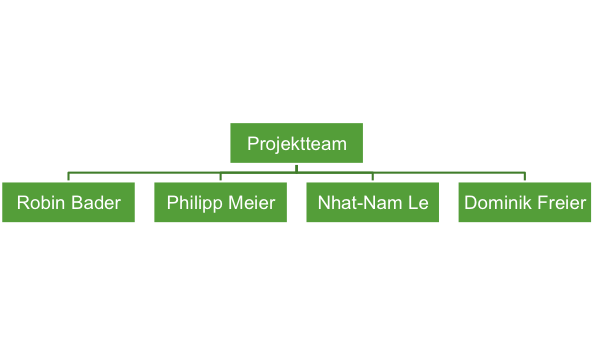
\includegraphics[width=0.8\textwidth]{content/images/projekt_organisation.png}
    \caption{Projekt Organisation}
\end{figure}

\section{Organisationsstruktur}
Nachfolgend die involvierten Personen und ihre Funktionen.
    \begin{table}[H]
        \tablestyle
        \tablealtcolored
        \begin{tabularx}{\textwidth}{l X X l}
        \tableheadcolor
            \tablehead Name & 
            \tablehead Funktion(en) & 
            \tablehead Kontakt & 
            \tablehead Bemerkungen \\  
        \tablebody
            Dominik Freier & Software-Entwickler & \href{mailto:dfreier@hsr.ch}{dfreier@hsr.ch} & \tabularnewline 
            Nhat-Nam Le & Software-Entwickler \linebreak Serveradministrator & \href{mailto:nle@hsr.ch}{nle@hsr.ch} & \tabularnewline 
            Philipp Meier & Software-Entwickler & \href{mailto:p1meier@hsr.ch}{p1meier@hsr.ch} & \tabularnewline 
            Robin Bader & Software-Entwickler & \href{mailto:r1bader@hsr.ch}{r1bader@hsr.ch} & \tabularnewline 
        \tableend
        \end{tabularx} 
    \end{table}

\section{Externe Schnittstellen}
\textbf{Betreuer:} Luc Bläser
\\
\textbf{Weitere Betreuer:} Hans Rudin und Daniel Keller

Herr Bläser wird das Projekt betreuen und Reviews durchführen. Für Fragen oder andere Anliegen können auch die übrigen Anspruchspersonen zu Rate gezogen werden.

    \chapter{Management Abläufe}

\section{Kostenvoranschlag}
\begin{itemize}
    \item Vier Entwickler während 14 Wochen
    \item Projektstart am 20. Februar 2014
    \item Projektende am 28. Mai 2014
    \item Aufwand Total: 14 Wochen * 10 Stunden * 8 Entwickler = 560 Stunden
\end{itemize}
Werden die Kernfunktionalitäten vorzeitig erfüllt, kann durch den Projektumfang die restliche Zeit vollumfänglich für optionale Funktionalitäten genutzt werden.

\section{Zeitliche Planung}
Wir werden in unserem Projekt nach dem Unified Process arbeiten. Die beinhaltet die Phasen: 
\\\begin{itemize}
    \item Inception
    \item Elaboration
    \item Construction
    \item Transition
\end{itemize}
\begin{figure}[ht]
    \center
    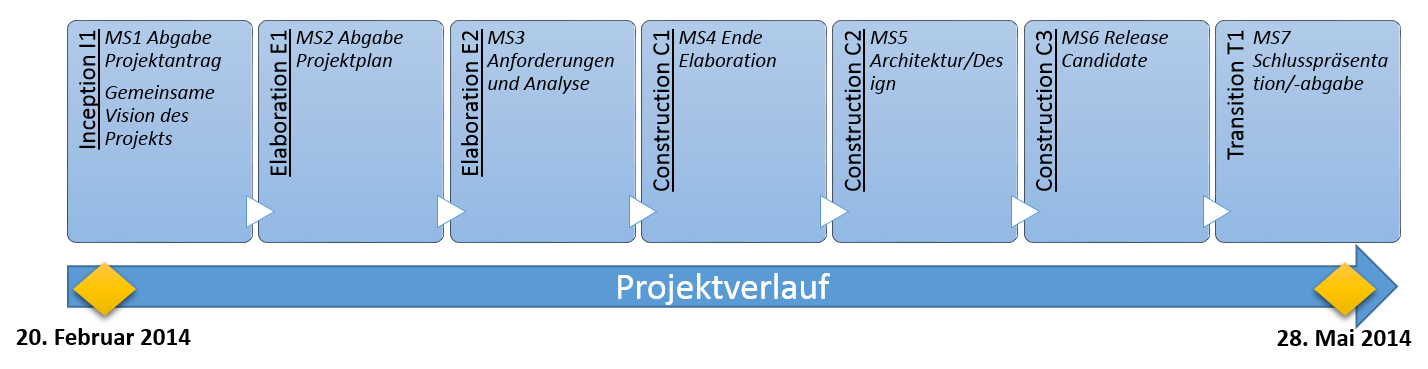
\includegraphics[width=\textwidth]{content/images/projektverlauf.png}
    \caption{Unified Process Phasen}
\end{figure}

\section{Iterationsplanung}
\begin{table}[H]
    \tablestyle
    \tablealtcolored
    \begin{tabularx}{\textwidth}{l X p{3.5cm} r}
        \tableheadcolor
            \tablehead Iteration &
            \tablehead Arbeitspaket &
            \tablehead Meilenstein &
            \tablehead SW \tabularnewline
        \tablebody
            \textit{Inception I1} &
            \begin{itemize}
                \item Projektantrag erstellen
                \item Virtueller Server beantragen
                \item Projektplan erstellen
                \item Entwicklungsumgebung einrichten (Client)
                \item Entwicklungsumgebung einrichten (Server)
                \item Vorgabe für Dokumentation erstellen
            \end{itemize} &
            \begin{itemize}
                \item MS1 Abgabe Projektantrag
                \item Gemeinsame Vision des Projekts
            \end{itemize} &
            1-2
        \tabularnewline
            \textit{Elaboration E1} &
            \begin{itemize}
                \item Projektplan verfeinern
                \item Domainanalyse
                    \begin{itemize}
                        \item Domainmodell
                        \item System State Diagramm
                        \item Operation Contracts
                    \end{itemize}
                \item Erstellen von Use Cases 
                    \begin{itemize}
                        \item Analyse
                        \item „brief“-Format zu 80%
                        \item „fully dressed“-Format zu 10%
                    \end{itemize}
                \item Erstellung Personas / Szenarios
                \item Anforderungsspezifikation erstellen
                \item Erstellung des Prototyps
                \item Machbarkeitsanalyse erstellen
            \end{itemize} &
            \begin{itemize}
                \item Abgabe MS2-RV. Projektplan
            \end{itemize} &
            2-4
        \tabularnewline
            \textit{Elaboration E2} &
            \begin{itemize}
                \item Entwicklungsumgebung vollständig eingerichtet
                \item Domainanalyse abgeschlossen
                \item Fertigstellung Anforderungsspezifikationen
                \item Fertigstellung Use Cases
                \item Fertigstellung Architektur-Prototyps
            \end{itemize} &
            \begin{itemize}
                \item MS3-RV. Anforderungen und Analyse
            \end{itemize} &
            5-6
        \tabularnewline
            \textit{Construction C1} &
            \begin{itemize}
                \item Implementationsarbeiten beginnen
                    \begin{itemize}
                        \item Login-/Logout-Funktion
                        \item Einsatzkatalog 
                        \item Mitgliederverwaltung
                    \end{itemize}
                \item Anpassungen gemäss Designreview
            \end{itemize} &
            \begin{itemize}
                \item MS4-RV. Ende Elaboration
            \end{itemize} &
            7-8
        \tabularnewline
        \tableend
    \end{tabularx}
    \caption{Iterationsplanung (1/2)}
\end{table}

\begin{table}[H]
    \tablestyle
    \tablealtcolored
    \begin{tabularx}{\textwidth}{l X p{3.5cm} r}
        \tableheadcolor
            \tablehead Iteration &
            \tablehead Arbeitspaket &
            \tablehead Meilenstein &
            \tablehead SW \tabularnewline
        \tablebody
            \textit{Construction C2} &
            \begin{itemize}
                \item Externes Design anpassen
                \item Implementationen erweitern
                    \begin{itemize}
                        \item Helfereinsätze importieren
                        \item Einsatzverwaltung
                    \end{itemize}
            \end{itemize} &
             &
            9-10
        \tabularnewline
            \textit{Construction C3} &
            \begin{itemize}
                \item Implementationen abschliessen
                    \begin{itemize}
                        \item Import- / Export-Funktionen
                        \item Optionale Funktionalitäten
                    \end{itemize}
                \item Testing 
                \item Reserven für Risiken
            \end{itemize} &
            \begin{itemize}
                \item MS5-RV. Architektur/Design
            \end{itemize} &
            11-12
        \tabularnewline
            \textit{Transition T1} &
            \begin{itemize}
                \item Präsentation vorbereiten
                \item Abschlussbericht verfassen
            \end{itemize} &
            \begin{itemize}
                \item MS6 Schlusspräsentation/-abgabe
            \end{itemize} &
            13-14
        \tabularnewline
        \tableend
    \end{tabularx}
    \caption{Iterationsplanung (2/2)}
\end{table}

\section{Meilensteine}

\subsection{MS1 Abgabe Projektantrag}
\begin{table}[H]
    \tablestyle
    \tablealtcolored
    \begin{tabularx}{\textwidth}{l X}
        \tablebody
        \tablehead Termin &
            21.02.14 (SW01) \tabularnewline
        \tablehead Phase &
            I1 \tabularnewline
        \tablehead Beschreibung  &
            Einreichung des Projektantrags und Genehmigung
            \tabularnewline
        \tablehead Deliverables  &
        	\begin{itemize}
                \item Projektantrag
            \end{itemize}
            \tabularnewline
        \tableend
    \end{tabularx}
    \caption{MS1 Abgabe Projektantrag}
\end{table}

\subsection{MS2 Abgabe Projektplan}
\begin{table}[H]
    \tablestyle
    \tablealtcolored
    \begin{tabularx}{\textwidth}{l X}
        \tablebody
        \tablehead Termin &
            06.03.14 (SW03) \tabularnewline
        \tablehead Phase &
            E1 \tabularnewline
        \tablehead Beschreibung  &
            Review Projektplan mit Zeitplan und aktuellen Iterationsplänen \tabularnewline
        \tablehead Deliverables  &
        	\begin{itemize}
                \item Projektplan mit Arbeitspaketen
            \end{itemize}
            \tabularnewline
        \tableend
    \end{tabularx}
    \caption{MS2 Abgabe Projektplan}
\end{table}

\subsection{MS3 Anforderungen und Analyse}
\begin{table}[H]
    \tablestyle
    \tablealtcolored
    \begin{tabularx}{\textwidth}{l X}
        \tablebody
        \tablehead Termin &
            13.03.14 (SW04) \tabularnewline
        \tablehead Phase &
            E2
            \tabularnewline
        \tablehead Beschreibung  &
            Review der Anforderungsspezifikation und Analyse \tabularnewline
        \tablehead Deliverables  &
        	\begin{itemize}
                \item Anforderungsanalyse
                \item Use-Case in Brief-Format
                \item Domainmodel
                \item Issues/Tasks in JIRA
            \end{itemize}
            \tabularnewline
        \tableend
    \end{tabularx}
    \caption{MS3 Anforderungen und Analyse}
\end{table}

\subsection{MS4 Ende Elaboration}
\begin{table}[H]
    \tablestyle
    \tablealtcolored
    \begin{tabularx}{\textwidth}{l X}
        \tablebody
        \tablehead Termin &
            27.03.14 (SW06) \tabularnewline
        \tablehead Phase &
            C1 \tabularnewline
        \tablehead Beschreibung  &
            Review der Dokumente und vorhandenen Code aus E1 \& E2 \tabularnewline
        \tablehead Deliverables  &
        	\begin{itemize}
                \item Architektur-Prototyp
            \end{itemize}
            \tabularnewline
        \tableend
    \end{tabularx}
    \caption{MS4 Ende Elaboration}
\end{table}

\subsection{MS5 Architektur/Design}
\begin{table}[H]
    \tablestyle
    \tablealtcolored
    \begin{tabularx}{\textwidth}{l X}
        \tablebody
        \tablehead Termin &
            01.05.14 (SW11) \tabularnewline
        \tablehead Phase &
            C3 \tabularnewline
        \tablehead Beschreibung  &
           Review der Architektur/Design \tabularnewline
        \tablehead Deliverables  &
        	\begin{itemize}
                \item Dokument Architektur/Design
                \item Testplan
                \item Code RC Version
                \item Protokoll Code\-Reviews
            \end{itemize}
            \tabularnewline
        \tableend
    \end{tabularx}
    \caption{MS5 Architektur/Design}
\end{table}

\subsection{MS6 Schlusspräsentation/-abgabe}
\begin{table}[H]
    \tablestyle
    \tablealtcolored
    \begin{tabularx}{\textwidth}{l X}
        \tablebody
        \tablehead Termin &
            28.05.2013 (SW14) \tabularnewline
        \tablehead Phase &
            T1
            \tabularnewline
        \tablehead Beschreibung  &
            Durchführung der Schlusspräsentation \tabularnewline
        \tablehead Deliverables  &
        	\begin{itemize}
                \item Finales Produkt
                \item Präsentation
                \item Abgabe der Resultate
            \end{itemize}
            \tabularnewline
        \tableend
    \end{tabularx}
    \caption{MS6 Schlusspräsentation/-abgabe}
\end{table}

\section{Besprechungen}
Es wird wöchentlich mindestens eine fixe Teamsitzung mit allen Projektbeteiligten durchgeführt. Diese wird jeweils am Donnerstag stattfinden und zwischen ein bis zwei Stunden andauern. 
\\Sie dienen dem Zweck, getätigte Arbeiten mitzuteilen, bevorstehende Arbeiten gemeinsam zu planen und offene Fragen zu beantworten. Falls nötig, können weitere Sitzungen einberufen werden. 
\\Protokolle werden jeweils auf \href{http://www.minutes.io}{www.minutes.io} geführt und per E-mail an alle Projektmitarbeiter verteilt.
\\\begin{enumerate}
	\item Was haben wir erledigt?
	\item Welche nächsten Schritte stehen an?
	\item Wo gibt oder gab es Probleme, welche Entscheidungen wurden getroffen?
\end{enumerate}
Für Kurznachrichten im Team wird mit WhatsApp kommuniziert.

    \chapter{Risikomanagement}

\section{Risiken}

\begin{table}[H]
    \tablestyle
    \tablealtcolored
    \begin{tabularx}{\textwidth}{l p{2cm} X c c c X X}
        \tableheadcolor
            \tablehead Nr &
            \tablehead Titel &
            \tablehead Beschreibung &
            \tablehead\rotatebox{90}{max. Schaden [h]} &
            \tablehead\rotatebox{90}{Eintrittswahrscheinlichkeit} &
            \tablehead\rotatebox{90}{Gewichteter Schaden} &
            \tablehead Vorbeugung &
            \tablehead \rotatebox{90}{\parbox[b]{3cm}{Verhalten beim Eintreten}}
        \tabularnewline
        \tableend
        \tablebody
            \textit{R1} &
            Microsoft-Technologien &
            Der Umgang mit Microsofts Web-Entwicklungs Tools ist für einige Teammitglieder neu. Möglicherweise kann nicht das gesamte Team mit voller Produktivität arbeiten. &
            48 &
            25\% &
            12 &
            Kontinuierliches Aneignen von Know-How durch Tutorials und Dokumentationsseiten von Microsoft nach Absprache mit erfahrenen Teammitgliedern. Dies geschieht in der Elaborationsphase. &
            Erfahrene Entwickler kümmern sich um die besonders anspruchsvollen und technologieabhängigen Arbeitspakete. 
        \tabularnewline
            \textit{R2} &
            Webservice Verfügbarkeit &
            Ein verwendeter Webservice verhält sich nicht erwartungskonform. Es könnte passieren, dass ein Service ausfällt oder fehlerhafte Daten liefert. &
            30 &
            5\% &
            1.5 &
            Layering der Komponenten für Datenimport. &
            Unteren Layer austauschen, sodass Daten von einer alternativen Ressource importiert werden können.
        \tabularnewline
            \textit{R3} &
            Team Foundation Server &
            TFS-Workflow lässt sich nicht auf das Projekt anwenden. Deployment- und Entwicklungsprozesse sind zu komplex, bzw. stehen nicht im Kosten-/Nutzenverhältnis. &
            30 &
            20\% &
            6 &
            In der Elaborationsphase eine Arbeitsumgebung mit TFS einrichten und überprüfen, ob die gängigen Szenarien im Entwicklungsprozess umsetzbar sind. Zusätzlich Rücksprache mit Herrn Bläser nehmen. &
            Verzicht auf TFS, Umstieg auf Jenkins, NANT
        \tabularnewline
    \tableend
    \end{tabularx}
    \caption{Technische Risiken (1/2)}
\end{table}
\begin{table}[H]
    \tablestyle
    \tablealtcolored
    \begin{tabularx}{\textwidth}{l p{2cm} X c c c X X}
        \tableheadcolor
            \tablehead Nr &
            \tablehead Titel &
            \tablehead Beschreibung &
            \tablehead\rotatebox{90}{max. Schaden [h]} &
            \tablehead\rotatebox{90}{Eintrittswahrscheinlichkeit} &
            \tablehead\rotatebox{90}{Gewichteter Schaden} &
            \tablehead Vorbeugung &
            \tablehead Verhalten beim Eintreten
        \tabularnewline
        \tableend
        \tablebody
            \textit{R4} &
            Virtueller Server &
            Kapazität/Leistung des Servers reicht nicht für das Projekt aus. &
            8 &
            10\% &
            0.8 &
            Systemanforderungen an TFS + Datenbankserver überprüfen. &
            Mehr Ressourcen fordern.
        \tabularnewline
            \textit{R5} &
            Webservice API &
            Die API eines verwendeten Webservice ändert sich im Verlauf des Projekts. &
            8 &
            5\% &
            0.4 &
            Abstraktion der API durch den Einsatz von flexiblem Software-Design. Schreiben eines kleinen Prototypen für die Benutzung der Webservices, um Probleme bereits in der Ellaborationsphase zu erkennen. &
            Neuen Adapter für API schreiben.
        \tabularnewline
            \textit{R6} &
            Datenverlust &
            Die gesamte geleistete Arbeit geht verloren. &
            480 &
            1\% &
            4.8 &
            Backups des Codes ausserhalb von TFS am Ende jeder Iteration. Dokumentation aller ausgeführten Schritte. &
            Anhand von restlichen Daten und Dokumentation noch einmal neu anfangen.
        \tabularnewline
            \textit{R7} &
            Architekturrisiken &
            In der Construction-Phase stellt sich heraus, dass die Requirements teils nicht sinnvoll bzw. anwendbar sind. &
            32 &
            15\% &
            4.8 &
            Prototypen erstellen und Architektur-/Designentscheide bereits in der Elaborationsphase treffen und Grundgerüst implementieren. &
            Abwägen, ob Kompromisse gemacht werden können oder nicht. Falls nicht, müssen grundlegende Änderungen am Produkt vorgenommen werden.
        \tabularnewline
            \textit{R8} &
            Wissen auf eine Person konzentriert &
            Das Wissen über Key-Parts ist auf eine Person konzentriert. Fällt diese aus, wird Zeit benötigt um das Wissen zu transferieren. &
            24 &
            25\% &
            6 &
            Am Ende jeder Iteration Wissen austauschen und sicherstellen, dass alle Teammitglieder verstehen was gemacht wurde. &
            Möglichst schnell alle relevanten Informationen besorgen, um die Weiterarbeit am Projekt zu ermöglichen.
        \tabularnewline 
            \multicolumn{3}{l}{\textbf{Summe}} &
            \textbf{660} &
             &
            \textbf{36,3} &
             &
        \tabularnewline
    \tableend
    \end{tabularx}
    \caption{Technische Risiken (2/2)}
\end{table}

\section{Umgang mit Risiken}
Die beschriebenen Risiken sind aufgrund einer ersten Einschätzung aufgestellt.
Jeweils zu Beginn einer neuen Iteration werden die Risiken neu betrachtet und beurteilt. Möglicherweise lassen sich im Verlauf des Projekts einige Risiken ausschliessen oder neue kommen hinzu.

    \chapter{Arbeitspakete}

\begin{table}[H]
    \tablestyle
    \tablealtcolored
    \begin{tabularx}{\textwidth}{Xllcr}
        \tableheadcolor
            \tablehead Name &
            \tablehead Kategorie &
            \tablehead Iteration &
            \tablehead Priorität &
            \tablehead Soll in Stunden
        \tabularnewline
        \tablebody
	    Latex Umgebung einrichten & Dokumentation & Inception 1 & 3     & 4 \tabularnewline
	    Latex Dokumentengerüst erstellen & Dokumentation & Inception 1 & 3     & 2 \tabularnewline
	    Dokumentvorlagen & Dokumentation & Inception 1 & 3     & 2 \tabularnewline
	    Visual Studio Online einrichten & Entwicklungsumgebung & Inception 1 & 2     & 2 \tabularnewline
	    Source Control einrichten & Entwicklungsumgebung & Inception 1 & 2     & 2 \tabularnewline
	    MSSQL Installieren & Implementation & Inception 1 & 2     & 2 \tabularnewline
	    Projektplan erstellen & Projektmanagement & Inception 1 & 1     & 8 \tabularnewline
	    Projektantrag & Projektmanagement & Inception 1 & 1     & 2 \tabularnewline
	    Iterationsplan & Projektmanagement & Inception 1 & 2     & 2 \tabularnewline
	    Risikomanagement & Projektmanagement & Inception 1 & 2     & 4 \tabularnewline
	    Projektsitzung & Projektmanagement & Inception 1 & 3     & 2 \tabularnewline
	    Domainmodell erstellen & Analyse & Elaboration 1 & 1     & 3 \tabularnewline
	    GUI Designs erstellen & Analyse & Elaboration 1 & 2     & 6 \tabularnewline
	    Domainanalyse & Analyse & Elaboration 1 & 2     & 2 \tabularnewline
	    Personas / Szenarios & Analyse & Elaboration 1 & 2     & 3 \tabularnewline
	    Operation Contract & Analyse & Elaboration 1 & 2     & 2 \tabularnewline
	    System State Diagram & Analyse & Elaboration 1 & 3     & 2 \tabularnewline
	    System Sequenz Diagram & Analyse & Elaboration 1 & 3     & 4 \tabularnewline
	    Activity Diagram & Analyse & Elaboration 1 & 2     & 4 \tabularnewline
    \tableend
    \end{tabularx}
    \caption{Arbeitspakete (1/3)}
\end{table}

\begin{table}[H]
    \tablestyle
    \tablealtcolored
    \begin{tabularx}{\textwidth}{Xllcr}
        \tableheadcolor
            \tablehead Name &
            \tablehead Kategorie &
            \tablehead Iteration &
            \tablehead Priorität &
            \tablehead Soll in Stunden
        \tabularnewline
        \tablebody
	    Logische Architektur & Design & Elaboration 1 & 1     & 4 \tabularnewline
	    Internes Design & Design & Elaboration 1 & 1     & 4 \tabularnewline
	    Prototypen & Implementation & Elaboration 1 & 2     & 8 \tabularnewline
	    Zeitplanung erstellen & Projektmanagement & Elaboration 1 & 3     & 2 \tabularnewline
	    Use Case in Brief Format & Requirements & Elaboration 1 & 2     & 4 \tabularnewline
	    Anforderungsspezifikationen & Requirements & Elaboration 1 & 2     & 4 \tabularnewline
	    Datenbankmodell erstellen &  Entwicklungsumgebung & Elaboration 1 & 1     & 4 \tabularnewline
	    Projektsitzung & Projektmanagement & Elaboration 1 & 3     & 2 \tabularnewline
	    Machbarkeitsanalyse & Projektmanagement & Elaboration 1 & 2     & 4 \tabularnewline
	    Externes Design & Analyse & Elaboration 2 & 2     & 6 \tabularnewline
	    Deployment einrichten & Entwicklungsumgebung & Elaboration 2 & 2     & 4 \tabularnewline
	    Testumgebung einrichten & Entwicklungsumgebung & Elaboration 2 & 2     & 4 \tabularnewline
	    Automatisches Testing & Entwicklungsumgebung & Elaboration 2 & 2     & 4 \tabularnewline
	    Automatisches Building & Entwicklungsumgebung & Elaboration 2 & 2     & 4 \tabularnewline
	    Visual Studio für Deployment konfigurieren & Entwicklungsumgebung & Elaboration 2 & 1     & 4 \tabularnewline
	    Einrichten Infrastruktur & Implementation & Elaboration 2 & 1     & 8 \tabularnewline
	    IIS Konfigurieren & Implementation & Elaboration 2 & 1     & 2 \tabularnewline
	    Use Case in Fully Dressed Format & Requirements & Elaboration 2 & 3     & 6 \tabularnewline
	    Projektsitzung & Projektmanagement & Elaboration 2 & 3     & 2 \tabularnewline
	    Loginfunktion & Implementation & Construction 1 & 2     & 4 \tabularnewline
    \tableend
    \end{tabularx}
    \caption{Arbeitspakete (2/3)}
\end{table}

\begin{table}[H]
    \tablestyle
    \tablealtcolored
    \begin{tabularx}{\textwidth}{Xllcr}
        \tableheadcolor
            \tablehead Name &
            \tablehead Kategorie &
            \tablehead Iteration &
            \tablehead Priorität &
            \tablehead Soll in Stunden
        \tabularnewline
        \tablebody
	    Logoutfunktion & Implementation & Construction 1 & 2     & 2 \tabularnewline
	    Events anzeigen & Implementation & Construction 1 & 1     & 4 \tabularnewline
	    Eventdetails anzeigen & Implementation & Construction 1 & 2     & 2 \tabularnewline
	    Benutzerverwaltung CRUD & Implementation & Construction 1 & 1     & 6 \tabularnewline
	    Logging & Implementation & Construction 1 & 4     & 3 \tabularnewline
	    Bugfixing & Implementation & Construction 1 & 2     & 3 \tabularnewline
	    Code-Review & Qualitätsmanagement & Construction 1 & 4     & 2 \tabularnewline
	    Usability Tests & Qualitätsmanagement & Construction 1 & 4     & 2 \tabularnewline
	    Projektsitzung & Projektmanagement & Construction 1 & 3     & 2 \tabularnewline
	    Helfereinsätze für Event anzeigen & Implementation & Construction 2 & 2     & 4 \tabularnewline
	    Helfereinsatz anmelden & Implementation & Construction 2 & 1     & 2 \tabularnewline
	    Helfereinsatz abmelden & Implementation & Construction 2 & 2     & 2 \tabularnewline
	    Helfereinsatzdetails anzeigen & Implementation & Construction 2 & 3     & 4 \tabularnewline
	    Einsätze von Mitgliedern anzeigen & Implementation & Construction 2 & 3     & 4 \tabularnewline
	    Events verwalten CRUD & Implementation & Construction 2 & 1     & 6 \tabularnewline
	    Helfereinsätze verwalten CRUD & Implementation & Construction 2 & 1     & 4 \tabularnewline
	    Helfereinsätze zuordnen & Implementation & Construction 2 & 2     & 4 \tabularnewline
	    Bugfixing & Implementation & Construction 2 & 2     & 3 \tabularnewline
	    Code-Review & Qualitätsmanagement & Construction 2 & 4     & 2 \tabularnewline
	    Usability Tests & Qualitätsmanagement & Construction 2 & 4     & 2 \tabularnewline
	    Projektsitzung & Projektmanagement & Construction 2 & 3     & 2 \tabularnewline
	    Events importieren (Verbands API) & Implementation & Construction 3 & 3     & 8 \tabularnewline
	    Mitglieder importieren (webling API) & Implementation & Construction 3 & 3     & 8 \tabularnewline
	    Bugfixing & Implementation & Construction 3 & 2     & 3 \tabularnewline
	    Code-Review & Qualitätsmanagement & Construction 3 & 4     & 2 \tabularnewline
	    Usability Tests & Qualitätsmanagement & Construction 3 & 4     & 2 \tabularnewline
	    Projektsitzung & Projektmanagement & Construction 3 & 3     & 2 \tabularnewline
    \tableend
    \end{tabularx}
    \caption{Arbeitspakete (3/3)}
\end{table}
    \chapter{Infrastruktur}

\section{Hardware}
Als Entwicklungsgeräte werden die einzelnen Notebooks der Projektmitarbeiter eingesetzt. Das Testing der Webapplikation soll ebenfalls auf den Geräten ausgeführt werden. Gehostet wird die Applikation auf einer virtuellen Maschine mit Windows Server 2012. Eingesetzt wird dafür die Infrastruktur der HSR.

\section{Software / Tools}
Für die Entwicklung wird Visual Studio 2013 eingesetzt. Mittels Visual Studio Online wird die Sourcecodeverwaltung vorgenommen und ebenfalls als Build-Server eingesetzt. Für die Datenpersistenz wird ein Microsoft SQL Server eingesetzt. Zum Hosting der Webapplikation setzen wir einen IIS Webserver ein.
\begin{figure}[h]
    \centering
    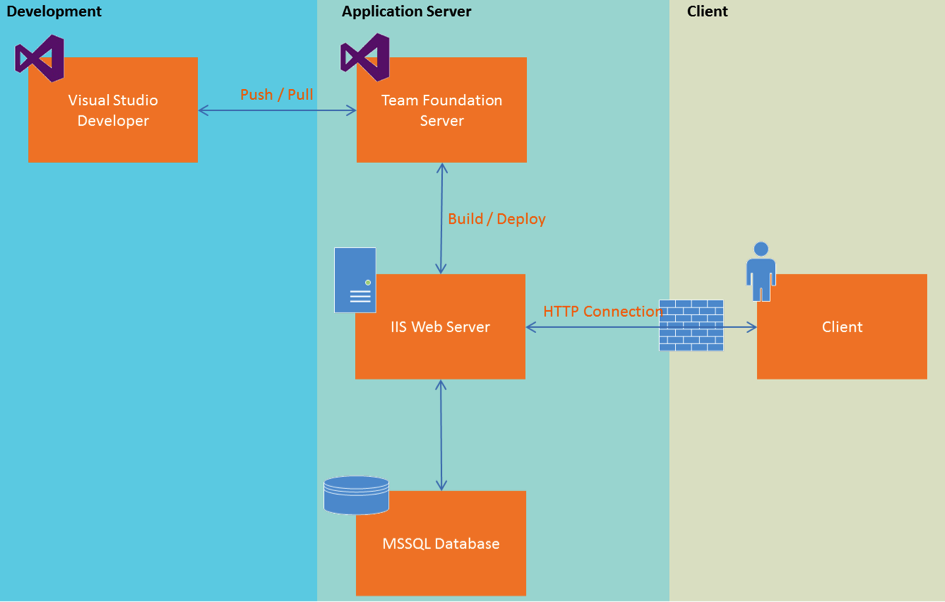
\includegraphics[width=0.8\textwidth]{content/images/infrastruktur.png}
    \caption{Infrastruktur}
\end{figure}

    \chapter{Qualitätsmassnahmen}

\section{Dokumentation}
Die Dokumentation wird in Latex erstellt und mit GIT als Versionskontrollsystem auf \href{https:www.//github.com}{GitHub} verwaltet. Dies bietet uns einige Vorteile zur Sicherstellung der Qualität der Dokumentation:
\\\begin{itemize}
    \item Gemeinsames bearbeiten mit Konfliktlösung (GIT)
    \item Automatische Versionierung des Dokumentes und Übersicht der Änderungen
    \item Eine zentrale Ablage für das Dokument
\end{itemize}


\section{Projektmanagement}
Als Projektmanagement Tool kommt \href{https://www.atlassian.com/software/jira/agile}{Atlassian JIRA} zum Einsatz. Sämtliche Ressourcen werden damit 
tracked und gemanaged. Die Arbeitspakete werden in JIRA erfassst, priorisiert, den Teammitgliedern zugeteilt und dann implementiert. 
Die JIRA-Instanz ist erreichbar über diese URL: 
\\\url{http://sinv-56086.edu.hsr.ch:40010}

\section{Entwicklung}
Der gesamte Quellcode des Projekts wird mithilfe des Team Foundation Servers verwaltet und versioniert. Wir setzen dabei auf das Cloud-Angebot von \href{http://www.visualstudio.com/}{Visual Studio Online} 
\\Es darf nur Code veröffentlicht werden, der einen sinnvollen Zwischenstand darstellt und der lauffähig und getestet ist.
\subsection{Vorgehen}

\subsection{Unit Testing}
Während der Entwicklung sollten für alle Funktionen, bei denen es sinnvoll ist, Unit-Tests durchgeführt. Bevor der Quellcode eingecheckt werden kann müssen diese Tests erfolgreich sein.
\\Das Bereitstellen eines möglichen Unit-Tests ist integraler Bestandteil eines Arbeitspaketes.
\begin{table}[H]
    \tablestyle
    \tablealtcolored
    \begin{tabularx}{\textwidth}{l X l}
        \tablebody
        \textbf{Unit Testing} &
            Während der Entwicklung sollten für alle Funktionen, bei denen es sinnvoll ist, Unit-Tests durchgeführt. Bevor der Quellcode eingecheckt werden kann müssen diese Tests erfolgreich sein.
            \tabularnewline
        \textbf{System Testing} &
            Nach jeder abgeschlossenen Iteration wird der aktuelle Build ausgiebig getestet. Daraus resultiert ein Testbericht. Aus den resultierenden Fehlern werden Incidents eröffnet.
            \tabularnewline
        \textbf{Usability Testing} &
            Um kontinuierlich externes Feedback zu erhalten und um die Bedienbarkeit zu testen, wird das Projekt nach jeder Iteration an ausgewählte Benutzer verteilt, um ihnen die Möglichkeit für Feedback zu geben. So können wir sicherstellen, dass das Endprodukt intuitiv bedient werden kann.
            \tabularnewline
        \tableend
    \end{tabularx}
    \caption{Unit Testing}
\end{table}

\subsection{Code Reviews}
Um die Motivation zur Erstellung von wartbarem Code und den Austausch von Programmiertechniken zu fördern, werden wir unseren Code gegenseitig Reviewen. Der Quellcode jedes Teammitglieds wird zum Review freigegeben und dabei von mindestens einem anderen Teammitglied kontrolliert. An gemeinsamen Code-Review-Sitzungen werden die Änderungsvorschläge durchgesprochen und in einem Review-Protokoll festgehalten.
\\ Folgende Kriterien werden untersucht:
\\\begin{itemize}
    \item Einhaltung der Code-Richtlinien
    \item Existenz von „Code Smells“
    \item Nachvollziehbarkeit des Codes
\end{itemize}


    % \input{template/playground}
    
    
\end{document}
